% Dit werk is gelicenseerd onder de licentie Creative Commons Naamsvermelding-GelijkDelen 4.0 Internationaal. Ga naar http://creativecommons.org/licenses/by-sa/4.0/ om een kopie van de licentie te kunnen lezen.
\chapter{Controlevolume's}
\label{sec:Controlevolume's}
%%%%%%%%%%%%%%%%%%%%%%%%%%%%%%%%%%%%%%%%%%%%%%%%%%%%%%%%%%%%%%%%%%%%%%%%%%%%%%%%%%%%%%%%%
\begin{toepassing}
	\label{buisaftap}
In een buis met een aftap met afmetingen zoals aangegeven op de figuur stroomt water.
		
Bepaal de gemiddelde stromingssnelheid in de aftap.

	\centering
	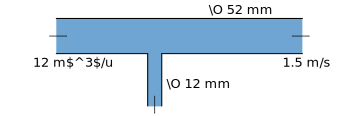
\includegraphics{fig/behoudsvergelijkingen/buisaftap}
\end{toepassing}
\begin{antwoord}{\ref{buisaftap}}
	$v = 1.3\unit{m/s}$
\end{antwoord}
%%%%%%%%%%%%%%%%%%%%%%%%%%%%%%%%%%%%%%%%%%%%%%%%%%%%%%%%%%%%%%%%%%%%%%%%%%%%%%%%%%%%%%%%%
\begin{toepassing}
	\label{jetski}
Bij een jetski wordt $0.05\unit{m^3/s}$ water aan de voorzijde aangezogen door een pomp en aan de achterzijde weer uitgestuwd. De opening aan de voorzijde is $0.006\unit{m^2}$ groot, aan de achterzijde $0.002\unit{m^2}$. Bepaal de kracht uitgeoefend door de aandrijving wanneer de jetski op zijn plaats wordt gehouden en de druk aan de voor en achterzijde gelijk is, de dichtheid van water mag $1000\unit{kg/m^3}$ verondersteld worden.

	\centering
	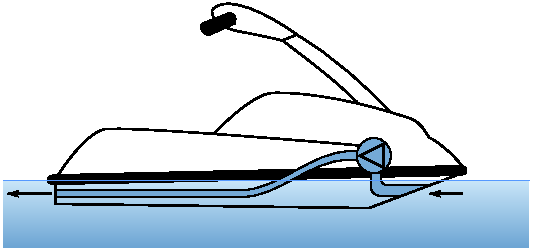
\includegraphics{fig/behoudsvergelijkingen/jetski}
\end{toepassing}
\begin{antwoord}{\ref{jetski}}
	$F = 833\unit{N}$
\end{antwoord}
%%%%%%%%%%%%%%%%%%%%%%%%%%%%%%%%%%%%%%%%%%%%%%%%%%%%%%%%%%%%%%%%%%%%%%%%%%%%%%%%%%%%%%%%%
\begin{toepassing}
	\label{turbojet}
Een stilstaande turbojet motor werkt met lucht. De inlaat heeft een oppervlakte van $2\unit{m^2}$, de gemiddelde snelheid is $100\unit{m/s}$ en de dichtheid is $1.22\unit{kg/m^3}$, aan de uitlaat is de snelheid $300\unit{m/s}$. In de motor wordt 2\% van het inlaat massadebiet aan brandstof massa ingespoten.

Bepaal de stuwkracht die de motor genereert als de druk aan de voor en achterzijde atmosfeerdruk is.

	\centering
	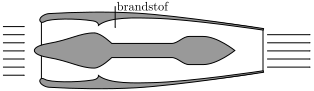
\includegraphics{fig/behoudsvergelijkingen/turbojet}
\end{toepassing}
\begin{antwoord}{\ref{turbojet}}
	$F = 50.3\unit{kN}$
\end{antwoord}
%%%%%%%%%%%%%%%%%%%%%%%%%%%%%%%%%%%%%%%%%%%%%%%%%%%%%%%%%%%%%%%%%%%%%%%%%%%%%%%%%%%%%%%%%
\begin{toepassing}
	\label{sluis}
Door een gedeeltelijk geopende sluis stroomt water met een dichtheid van $1000\unit{kg/m^3}$. Voor de sluis is de snelheid $1.2\unit{m/s}$ en de diepte 3 m. Na de sluis is de diepte nog 0.45 m.

Bepaal de kracht per meter breedte die nodig is om de sluis op zijn plaats te houden.

	\centering
	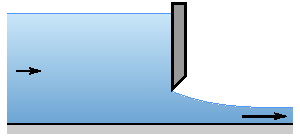
\includegraphics{fig/behoudsvergelijkingen/sluis}
\end{toepassing}
\begin{antwoord}{\ref{sluis}}
	$F = 18.7\unit{kN/m}$
\end{antwoord}
%%%%%%%%%%%%%%%%%%%%%%%%%%%%%%%%%%%%%%%%%%%%%%%%%%%%%%%%%%%%%%%%%%%%%%%%%%%%%%%%%%%%%%%%%
\begin{toepassing}
	\label{180gradenbocht}
Een flexibele afvoerleiding met een diameter van 22 mm en een lengte van 0.3 m maakt een verticale bocht van 180\deg als een omgekeerde U. De inlaat en uitlaat bevinden zich op gelijke hoogte en de leiding heeft een massa van 0.1 kg. Bepaal de kracht nodig om de bocht op zijn plaats te houden indien door de buis een water debiet ($\rho=1000\unit{kg/m^3}$) van 50 l/min stroomt, de uitlaat druk atmosfeerdruk is, en de stroming verliesvrij verondersteld mag worden.
\end{toepassing}
\begin{antwoord}{\ref{180gradenbocht}}
	$F = 1.55\unit{N}$
\end{antwoord}
%%%%%%%%%%%%%%%%%%%%%%%%%%%%%%%%%%%%%%%%%%%%%%%%%%%%%%%%%%%%%%%%%%%%%%%%%%%%%%%%%%%%%%%%%
\begin{toepassing}
	\label{afvoerbocht}
Een PVC bochtstuk van 90\deg voor afvoerleiding heeft een binnen diameter van 32 mm. De hartlijn heeft een straal van 20 mm. Door de buis stroomt water met een debiet van 40 l/min.
		
Als er geen drukverliezen optreden in de bocht en de druk aan de uitgang is atmosfeerdruk, bepaal dan de grootte en richting van de kracht die door de stroming uitgeoefend wordt op de buis.

	\centering
	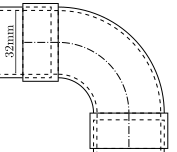
\includegraphics{fig/behoudsvergelijkingen/afvoerbocht}
\end{toepassing}
\begin{antwoord}{\ref{afvoerbocht}}
	$F_x = 0.55\unit{N}$, $F_y = 0.55\unit{N}$
\end{antwoord}
%%%%%%%%%%%%%%%%%%%%%%%%%%%%%%%%%%%%%%%%%%%%%%%%%%%%%%%%%%%%%%%%%%%%%%%%%%%%%%%%%%%%%%%%%
\begin{toepassing}[*]
	\label{waterstraal}
Bereken de kracht die een vrije stationaire waterstraal die loodrecht op een wand spuit op de wand uitoefent.

	\centering
	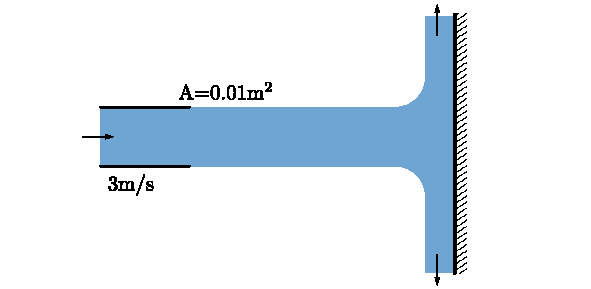
\includegraphics{fig/behoudsvergelijkingen/waterstraal}
\end{toepassing}
\begin{antwoord}{\ref{waterstraal}}
	$F = 90\unit{N}$
\end{antwoord}
%%%%%%%%%%%%%%%%%%%%%%%%%%%%%%%%%%%%%%%%%%%%%%%%%%%%%%%%%%%%%%%%%%%%%%%%%%%%%%%%%%%%%%%%%
\begin{toepassing}
	\label{dredger}
Een baggerboot zuigt een mengsel van water en zand op vanuit een rivierbodem en spuit dit door een uitlaat nozzle zoals afgebeeld op de figuur. De diameter van de uitlaat is 0.6 m en de snelheid is 12 m/s. Bepaal de kracht die de scheepsschroef moet leveren om de boot op zijn plaats te houden als de uitlaat onder een hoek van 30\deg\ met de horizontale staat en de dichtheid van het zand water mengsel $1400\unit{kg/m^3}$ bedraagt.

	\centering
	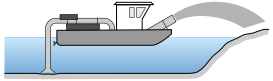
\includegraphics{fig/behoudsvergelijkingen/dredger}
\end{toepassing}
\begin{antwoord}{\ref{dredger}}
	$F = 49.4\unit{kN}$
\end{antwoord}
%%%%%%%%%%%%%%%%%%%%%%%%%%%%%%%%%%%%%%%%%%%%%%%%%%%%%%%%%%%%%%%%%%%%%%%%%%%%%%%%%%%%%%%%%
\begin{toepassing}[*]
	\label{45gradenbocht}
Een leiding met binnendiameter 300 mm ligt in een horizontaal vlak. In de leiding stroomt water aan een debiet van 0.25\unit{m^3/s}.

Bepaal de grootte en de richting van de kracht die op het bochtstuk inwerkt indien de overdruk voor de bocht 0.4 bar bedraagt. De zwaartekracht en viskeuze effecten mogen buiten beschouwing gelaten worden.

	\centering
	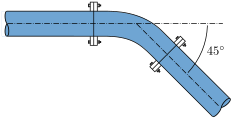
\includegraphics{fig/behoudsvergelijkingen/45gradenbocht}
\end{toepassing}
\begin{antwoord}{\ref{45gradenbocht}}
	$F_x = 1.09\unit{kN}$, $F_y = 1.37\unit{kN}$
\end{antwoord}
%%%%%%%%%%%%%%%%%%%%%%%%%%%%%%%%%%%%%%%%%%%%%%%%%%%%%%%%%%%%%%%%%%%%%%%%%%%%%%%%%%%%%%%%%
\begin{toepassing}[*]
	\label{verwijding}
Olie met een dichtheid van 800\unit{kg/m^3} stoomt met een debiet van 200 l/min door een verwijding met een inlaat diameter van 28 mm en een uitlaat diameter van 50 mm. De overdruk aan de inlaat is 1.00 bar, aan de uitlaat is de overdruk 1.06 bar.

Bepaal de grootte en richting van kracht die door de stroming op de verwijding uitgeoefend wordt.
\end{toepassing}
\begin{antwoord}{\ref{verwijding}}
	$F = 137\unit{N}$ tegengesteld aan de stromingsrichting
\end{antwoord}
%%%%%%%%%%%%%%%%%%%%%%%%%%%%%%%%%%%%%%%%%%%%%%%%%%%%%%%%%%%%%%%%%%%%%%%%%%%%%%%%%%%%%%%%%
\begin{toepassing}[*]
	\label{turbine}
Een hydraulische turbine onttrekt 600 MW arbeid aan een waterdebiet van 600\unit{m^3/s}. De inlaat van de turbine heeft een diameter van 8 m, de uitlaat een diameter van 10 m. Aan de inlaat van de turbine is de druk 10 bar. Het hoogteverschil tussen in- en uitlaat mag verwaarloosd worden en de stroming wordt verliesvrij verondersteld.

Bepaal de druk aan de uitlaat van de turbine.

	\centering
	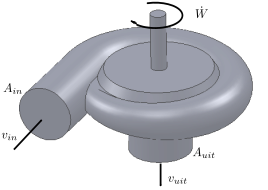
\includegraphics{fig/behoudsvergelijkingen/turbine}
\end{toepassing}
\begin{antwoord}{\ref{turbine}}
	$p = 0.4\unit{bar}$
\end{antwoord}

\section*{Antwoorden}
	\begin{multicols}{2}
		\includecollection{antwoorden}
	\end{multicols}